\subsection{Etude du lien entre temps de sommeil et habitudes alimentaires}

\subsubsection{Tableau de contingence et test chi-deux pour l'ensemble des individus}

Nous pouvons voir dans le tableau en figure \ref{tab:contTableDietarySleepAll} que les effectifs sont globalement équilibrés dans le sens où il y a environ autant de personnes ayant des habitudes alimentaires saines, modérées ou non saines, et de même pour le temps de sommeil. 
Le test chi-deux nous donne une p-valeur de environ $ 2\%$, ce qui indique que les 2 variables sont significativement corrélées. Ainsi, les persones ayant un régime alimentaire sain par exemple, pourront avoir tendance à adopter un certain type de sommeil.

\begin{figure}[!h]
    \begin{center}
      \begin{tabular}{|c|c|c|c|}
        \hline 
        & \multicolumn{3}{|c|}{Dietary Habits}\\ 
        \hline
        Sleep Duration & Healthy & Moderate & Unhealthy\\
        \hline 
        Less than 5 hours & 41 & 45 & 37 \\ 
        \hline 
        5-6 hours & 52 & 41 & 30\\
        \hline 
        7-8 hours & 37 & 44 & 47\\
        \hline 
        More than 8 hours & 31 & 41 & 55\\
        \hline
      \end{tabular}
    \end{center}
    \caption{Table de contingence entre le temps de sommeil et les habitudes alimentaires}
    \label{tab:contTableDietarySleepAll}
\end{figure}  

\subsubsection{Test chi-deux sur les individus dépressifs et non dépressifs}

Après exécution du test chi-deux sur les individus dépressifs, on obtient une p-valeur d'environ $ 33\%$, tandis que chez les personnes dépressives, on obtient environ $ 2\%$. Ainsi la dépendance n'est conservée que chez les personnes non dépressives. 

Cette indépendance chez les personnes dépressives met en avant l'origine multifactorielle de cette maladie qui perturbe l'ensemle des habitudes de vie. Cela peut conduire à de l'hypersomnie comme de l'insomnie, à une perte d'appétit ou du grignotage ce qui perturbe le lien habituel que l'on observe chez les personnes non dépressives qui ont des comportements alimentaires et des habitudes de sommeil plus stables et cohérents. 

La corrélation des non dépressifs pourrait compenser l'absence de corrélation chez les dépressifs et former la corrélation globale que l'on observe. 

\subsubsection{Etude des cercles de corrélation}

\begin{figure}[!h]
  \begin{center}
    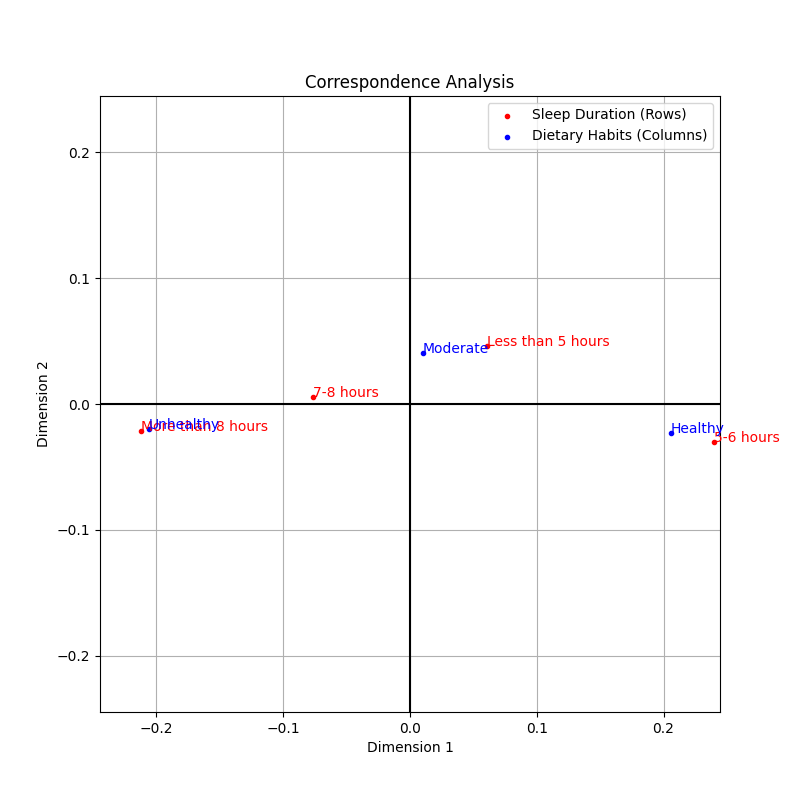
\includegraphics[width=0.55\textwidth]{Images/Sleep_Dietary_all/Corr_circle.png}
  \end{center}
  \caption{Cercle des corrélations de l'AFC entre le temps de sommeil et les habitudes alimentaires sur l'ensemble des individus}\label{fig:corrSleepDietaryAll}
\end{figure}

On observe dans la figure \ref{fig:corrSleepDietaryAll} un fort lien de corrélation d'une part entre les personnes ayant un temps de sommeil de 5-6 heures et des habitudes alimentaires saines, et d'autre part entre les personnes dormant beaucoup et mangeant de manière peu saine. Les autres points, trop proches du centre, ne sont pas interprétables dans cette étude. 

\begin{figure}[!h]
  \centering
  \begin{minipage}{0.45\textwidth}
    \centering
    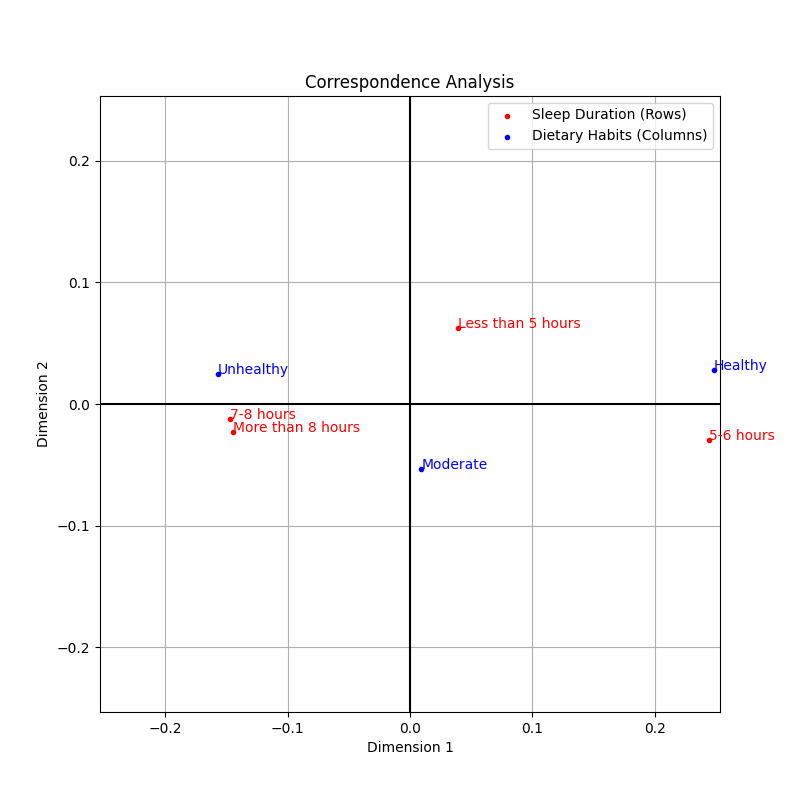
\includegraphics[width=\linewidth]{Images/Sleep_Dietary_depressive/Corr_circle.png}
  \end{minipage}\hfill
  \begin{minipage}{0.45\textwidth}
    \centering
    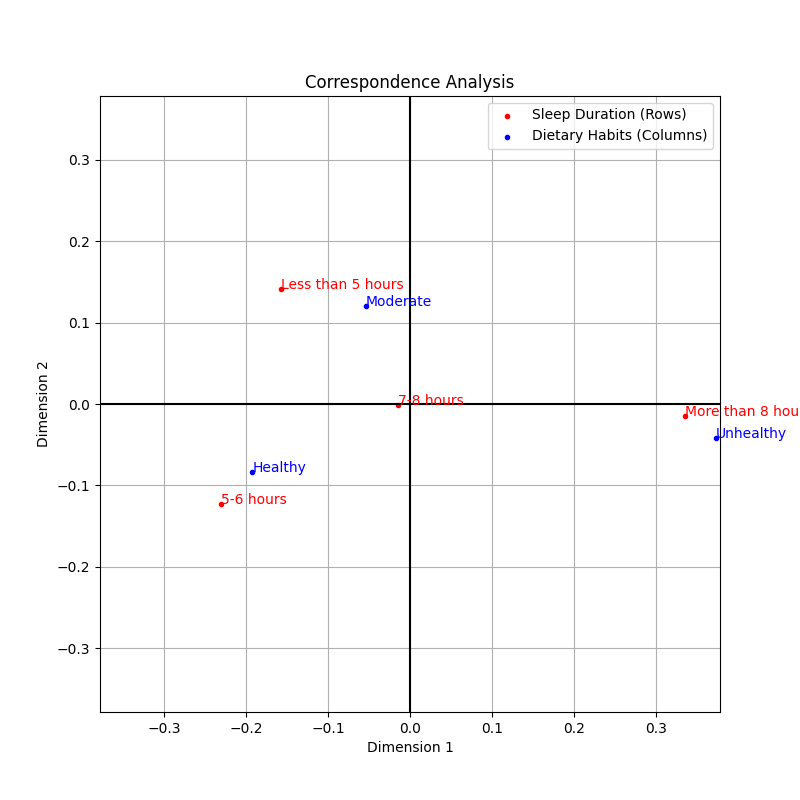
\includegraphics[width=\linewidth]{Images/Sleep_Dietary_non_depressive/Corr_circle.png}
  \end{minipage}  
  \caption{Cercles des corrélations de l'AFC entre le temps de sommeil et les habitudes alimentaires pour les dépressifs (à gauche) et les non dépressifs (à droite)}\label{fig:corrDietarySleep}
\end{figure}

De plus, que ce soit chez les personnes dépressives ou non dépressives, on remarque dans la figure \ref{fig:corrDietarySleep} que les tendances semblent persister, à la différence près que chez les dépressifs, les personnes dormant entre 7 et 8 heures tendent plus à avoir un mauvais régime alimentaire, et que chez les non dépressifs, le lien entre le régime sain et 5 à 6 heures de sommeil semble moins certains. 

Il serait intéressant de pouvoir observer si ces personnes sont sédentaires ou non. 
Des personnes sédentaires, qu’elles soient dépressives ou non, pourraient avoir perdu un intérêt pour la cuisine et consacreraient leur temps à dormir. Cela apparaît particulièrement cohérent chez les personnes dépressives qui, dans leurs phases de sédentarité, seraient enclines à de l’hypersomnie et des habitudes alimentaires peu saines comme du grignotage ou un manque d’attrait pour la cuisine. Ce comportement n’est pas non plus incohérent chez des personnes non dépressives mais qui présentent cependant une importante sédentarité. Un sommeil long peut être associé à un manque de dynamisme ou à une sédentarité souvent corrélés à un régime alimentaire peu sain.
A l’opposé du cercle, le manque de sommeil pourrait être associé à un mode de vie actif pouvant et voulant être compensé par une alimentation saine. Les personnes actives ont les finances et le dynamisme qui permet de mieux subvenir à leurs besoins alimentaires. Le groupe de personnes dépressives peut tout de même présenter des personnes dans la vie active d’où cette corrélation aussi dans leur effectif. Chez les personnes non dépressives, cette corrélation est probablement moins forte car leur état mental leur octroie une plus grande perméabilité dans leur rythme de vie. Elles ne vont pas nécessairement se diriger vers des comportements extrêmes.
Les comportements extrêmes sont les plus déterminants dans les corrélations observées.

\subsubsection{Contributions des variable dans les composantes principales}

\begin{figure}[H]
  \begin{center}
    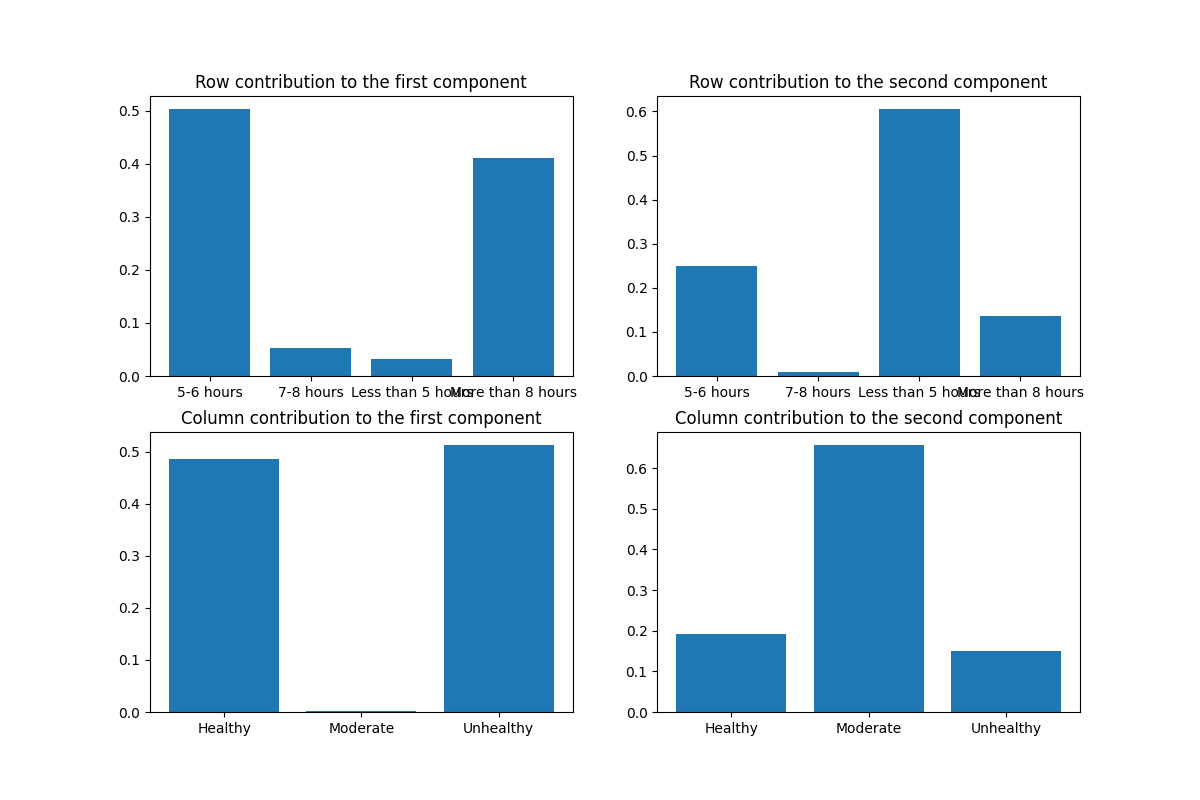
\includegraphics[width=0.65\textwidth]{Images/Sleep_Dietary_all/RowColumnsContributions.png}
  \end{center}
  \caption{Contributions des catégories de temps de sommeil et de qualité d'alimentation dans les composantes principales pour l'ensemble des individus}
  \label{fig:contribSleepDietaryAll}
\end{figure}

Sur l’effectif complet de la figure \ref{fig:contribSleepDietaryAll} la première composante était bien plus significative que la seconde, sa valeur propre étant 28 fois plus élevée. Elle capte l’essentiel de la variance des données. La seconde variable illustre des comportements plus résiduels.
Sur cette première composante, on observe le comportement décrit jusqu’à présent, les comportements extrêmes, pour le sommeil ou les habitudes alimentaires, représentent les contributions les plus importantes. Sur la seconde composante, on observe que les plus grandes contributions sont des comportements que l’on n’a pas réussi à lier à d’autres. Ceci est justifié par la bien moindre valeur de sa valeur propre associée.

\begin{figure}[H]
  \centering
  \begin{minipage}{0.5\textwidth}
    \centering
    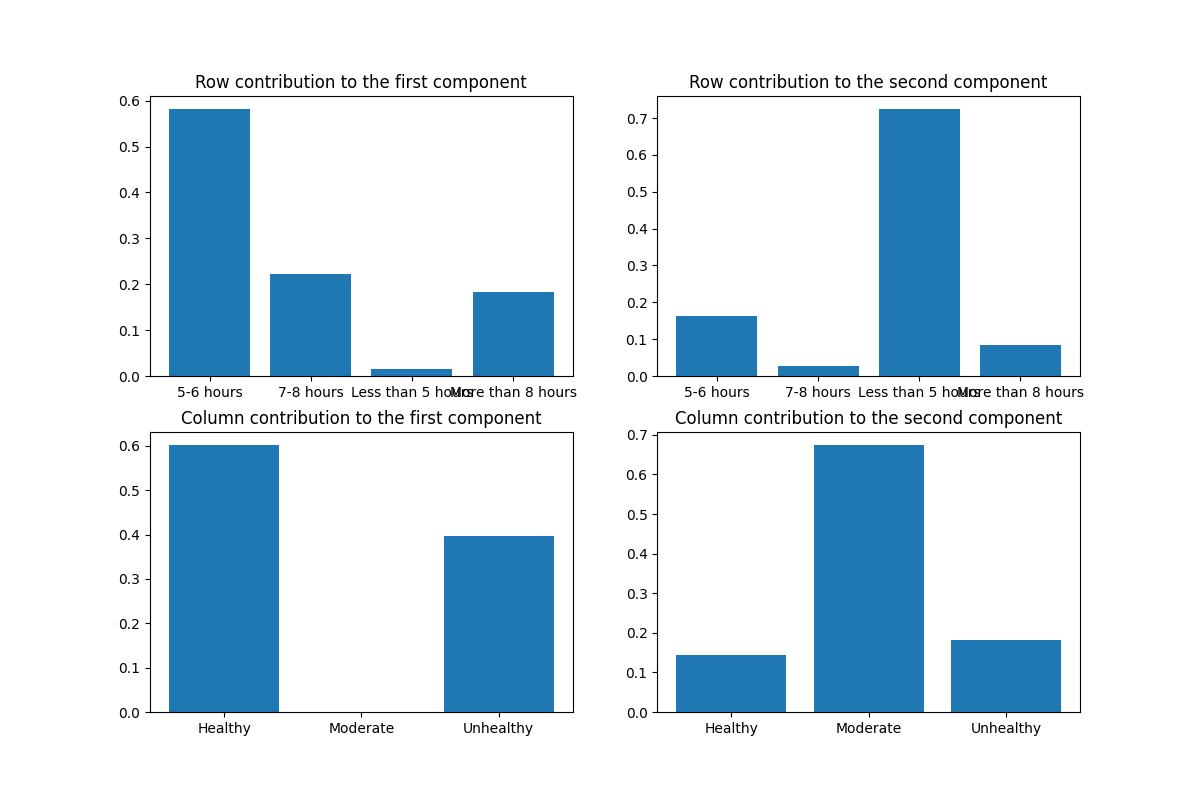
\includegraphics[width=\linewidth]{Images/Sleep_Dietary_depressive/RowColumnsContributions.png}
  \end{minipage}\hfill
  \begin{minipage}{0.5\textwidth}
    \centering
    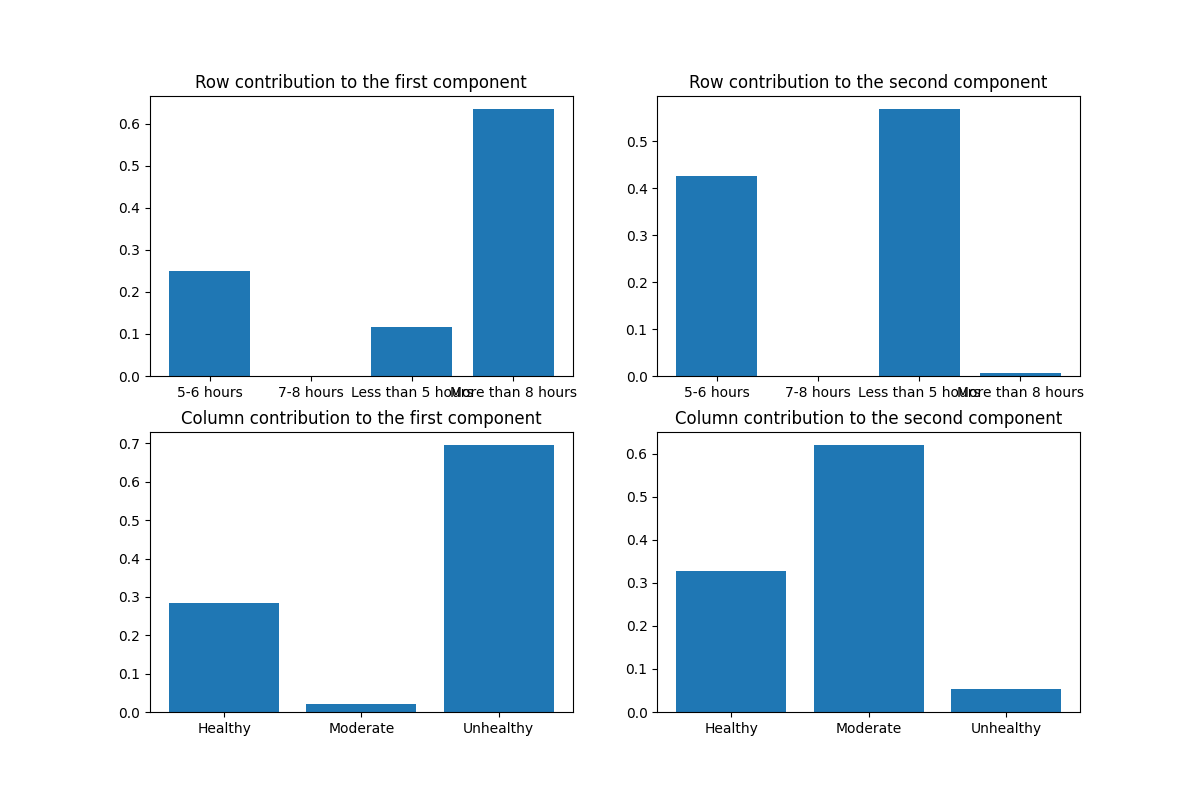
\includegraphics[width=\linewidth]{Images/Sleep_Dietary_non_depressive/RowColumnsContributions.png}
  \end{minipage}  
  \caption{Contributions des catégories de temps de sommeil et de qualité d'alimentation dans les composantes principales pour les dépressifs (à gauche) et les non dépressifs (à droite)}
  \label{fig:contribSleepDietary}
\end{figure}

Chez les personnes dépressives, selon la figure \ref{fig:contribSleepDietary},  la première composante, c’est l’association 5-6 heures de sommeil et régime healthy qui sont mises en avant dans les contributions. La seconde composante montre la même tendance que pour le groupe complet, soit une grande contribution de facteurs décorrélés des autres dans notre étude. C’est une observation que nous pouvons aussi faire chez les personnes non dépressives toujours d’après la figure \ref{fig:contribSleepDietary}. Cependant, pour la première composante, c’est à l’inverse le lien entre unhealthy et 8 heures de sommeil ou plus qui est mis en avant.

De manière générale, les comportements polarisés pourraient être associés à des profils typiques, bien définis. Par exemple, un comportement sédentaire pousse à une grande quantité de sommeil et des habitudes alimentaires malsaines et inversement pour un mode de vie plus actif. Ce sont deux modes de vie bien différenciés mais qui sont observés dans les effectifs dépressifs comme non dépressifs.
